% Notes:
% - Compare to Gaia RV error / RUWE
% - Cross-match to Kepler, K2, TESS 2 min cadence, show some examples
% - Short-period things: allude to Daunt et al. (in prep)?
% -

% Relevant papers:
% - Asteroseismic modes / RV: https://ui.adsabs.harvard.edu/abs/2020MNRAS.493.1388Y/abstract
% - https://ui.adsabs.harvard.edu/abs/2018MNRAS.480L..48Y/abstract

% \begin{figure}[!t]
% \begin{center}
% % \includegraphics[width=0.9\textwidth]{visitstats.pdf}
% {\color{red} Figure placeholder}
% \end{center}
% \caption{%
% TODO
% \label{fig:chiplots}
% }
% \end{figure}

\PassOptionsToPackage{usenames,dvipsnames}{xcolor}
\documentclass[modern]{aastex63}
% \documentclass[twocolumn]{aastex63}

% Load common packages
\usepackage{microtype}  % ALWAYS!
\usepackage{amsmath}
\usepackage{amsfonts}
\usepackage{amssymb}
\usepackage{booktabs}
\usepackage{graphicx}
% \usepackage{color}

\usepackage{enumitem}
\setlist[description]{style=unboxed}

% Hogg's issues
\renewcommand{\twocolumngrid}{\onecolumngrid} % guess what this does HAHAHA!
\setlength{\parindent}{1.1\baselineskip}
\addtolength{\topmargin}{-0.2in}
\addtolength{\textheight}{0.4in}
\sloppy\sloppypar\raggedbottom\frenchspacing

% For referee:
\newcommand{\changes}[1]{{\color{violet}#1}}

% Numbers:
\newcommand{\nsources}{\ensuremath{232\,495}}
% \newcommand{\Kmin}{M_{\rm min}}
% \newcommand{\Kminval}{512}
% \newcommand{\nbinary}{\ensuremath{19\,635}}

% \newcommand{\goldsample}{\textit{Gold Sample}}
% \newcommand{\ngold}{\ensuremath{1\,032}}
% \newcommand{\nbimodal}{\ensuremath{127}}

% Other
\newcommand{\visit}{visit}
\newcommand{\thisdr}{\dr{17}}

\graphicspath{{figures/}}
% \definecolor{cbblue}{HTML}{3182bd}
% \usepackage{hyperref}
% \definecolor{linkcolor}{rgb}{0.02,0.35,0.55}
% \definecolor{citecolor}{rgb}{0.45,0.45,0.45}
% \hypersetup{colorlinks=true,linkcolor=linkcolor,citecolor=citecolor,
%             filecolor=linkcolor,urlcolor=linkcolor}
% \hypersetup{pageanchor=true}

\newcommand{\documentname}{\textsl{Article}}
\newcommand{\sectionname}{Section}
\renewcommand{\figurename}{Figure}
\newcommand{\equationname}{Equation}
\renewcommand{\tablename}{Table}

% Missions
\newcommand{\project}[1]{\textsl{#1}}

% Packages / projects / programming
\newcommand{\package}[1]{\textsl{#1}}
\newcommand{\acronym}[1]{{\small{#1}}}
\newcommand{\github}{\package{GitHub}}
\newcommand{\python}{\package{Python}}
\newcommand{\emcee}{\project{emcee}}

% Stats / probability
\newcommand{\given}{\,|\,}
\newcommand{\norm}{\mathcal{N}}
\newcommand{\pdf}{\textsl{pdf}}

% Maths
\newcommand{\dd}{\mathrm{d}}
\newcommand{\transpose}[1]{{#1}^{\mathsf{T}}}
\newcommand{\inverse}[1]{{#1}^{-1}}
\newcommand{\argmin}{\operatornamewithlimits{argmin}}
\newcommand{\mean}[1]{\left< #1 \right>}

% Non-scalar variables
\renewcommand{\vec}[1]{\ensuremath{\bs{#1}}}
\newcommand{\mat}[1]{\ensuremath{\mathbf{#1}}}

% Unit shortcuts
\newcommand{\msun}{\ensuremath{\mathrm{M}_\odot}}
\newcommand{\mjup}{\ensuremath{\mathrm{M}_{\mathrm{J}}}}
\newcommand{\kms}{\ensuremath{\mathrm{km}~\mathrm{s}^{-1}}}
\newcommand{\mps}{\ensuremath{\mathrm{m}~\mathrm{s}^{-1}}}
\newcommand{\pc}{\ensuremath{\mathrm{pc}}}
\newcommand{\kpc}{\ensuremath{\mathrm{kpc}}}
\newcommand{\kmskpc}{\ensuremath{\mathrm{km}~\mathrm{s}^{-1}~\mathrm{kpc}^{-1}}}
\newcommand{\dayd}{\ensuremath{\mathrm{d}}}
\newcommand{\yr}{\ensuremath{\mathrm{yr}}}
\newcommand{\AU}{\ensuremath{\mathrm{AU}}}
\newcommand{\Kel}{\ensuremath{\mathrm{K}}}

% Misc.
\newcommand{\bs}[1]{\boldsymbol{#1}}

% Astronomy
\newcommand{\DM}{{\rm DM}}
\newcommand{\feh}{\ensuremath{{[{\rm Fe}/{\rm H}]}}}
\newcommand{\mh}{\ensuremath{{[{\rm M}/{\rm H}]}}}
\newcommand{\df}{\acronym{DF}}
\newcommand{\logg}{\ensuremath{\log g}}
\newcommand{\Teff}{\ensuremath{T_{\textrm{eff}}}}
\newcommand{\vsini}{\ensuremath{v\,\sin i}}
\newcommand{\mtwomin}{\ensuremath{M_{2, {\rm min}}}}

% TO DO
\newcommand{\todo}[1]{{\color{red} TODO: #1}}

\newcommand{\gaia}{\textsl{Gaia}}
\newcommand{\dr}[1]{\acronym{DR}#1}
\newcommand{\apogee}{\acronym{APOGEE}}
\newcommand{\sdss}{\acronym{SDSS}}
\newcommand{\sdssiv}{\acronym{SDSS-IV}}
\newcommand{\thejoker}{\project{The~Joker}}

\shorttitle{Close binaries in APOGEE DR17}
\shortauthors{Price-Whelan et al.}

\begin{document}

\title{Close Binary Companions in the APOGEE Survey Data Release 17: \\
       TODO}

\author[0000-0003-0872-7098]{Adrian~M.~Price-Whelan}
\affiliation{Center for Computational Astrophysics, Flatiron Institute,
             Simons Foundation, 162 Fifth Avenue, New York, NY 10010, USA}
\email{aprice-whelan@flatironinstitute.org}
\correspondingauthor{Adrian M. Price-Whelan}

% \author[0000-0003-2866-9403]{David~W.~Hogg}
% \affiliation{Center for Computational Astrophysics, Flatiron Institute,
%              Simons Foundation, 162 Fifth Avenue, New York, NY 10010, USA}
% \affiliation{Center for Cosmology and Particle Physics,
%              Department of Physics,
%              New York University, 726 Broadway,
%              New York, NY 10003, USA}
% \affiliation{Max-Planck-Institut f\"ur Astronomie,
%              K\"onigstuhl 17, D-69117 Heidelberg, Germany}

% \author[0000-0003-4996-9069]{Hans-Walter~Rix}
% \affiliation{Max-Planck-Institut f\"ur Astronomie,
%              K\"onigstuhl 17, D-69117 Heidelberg, Germany}


% % APOGEE:
% \author[0000-0002-1691-8217]{Rachael~L.~Beaton}
% \altaffiliation{Hubble Fellow}
% \altaffiliation{Carnegie-Princeton Fellow}
% \affiliation{Department of Astrophysical Sciences, Princeton University,
%              4 Ivy Lane, Princeton, NJ~08544}
% \affiliation{The Observatories of the Carnegie Institution for Science,
%              813 Santa Barbara St., Pasadena, CA~91101}

% \author[0000-0002-7871-085X]{Hannah~M.~Lewis}
% \affiliation{Department of Astronomy, University of Virginia,
%              Charlottesville, VA 22904-4325, USA}

% \author[0000-0002-1793-3689]{David~L.~Nidever}
% \affiliation{Department of Physics, Montana State University,
%              P.O. Box 173840, Bozeman, MT 59717-3840}
% \affiliation{NSF’s National Optical-Infrared Astronomy Research Laboratory,
%              950 North Cherry Ave, Tucson, AZ 85719}


% % APOGEE alphabetical:
% \author{Andr\'es~Almeida}
% \affiliation{Instituto de Investigaci\'on Multidisciplinario en Ciencia y
%              Tecnolog\'ia, Universidad de La Serena, Benavente 980,
%              La Serena, Chile}

% \author{Carles~Badenes}
% \affiliation{Department of Physics and Astronomy,
%              and Pittsburgh Particle Physics, Astrophysics and Cosmology Center
%              (PITT PACC), University of Pittsburgh, 3941 O’Hara Street,
%              Pittsburgh, PA 15260, USA}

% \author[0000-0003-1086-1579]{Rodolfo~Barba}
% \affiliation{Departamento de Astronom\'ia, Facultad de Ciencias,
%              Universidad de La Serena, Cisternas 1200, La Serena, Chile}

% \author{Timothy~C.~Beers}
% \affiliation{Department of Physics and JINA Center for the Evolution of the
%              Elements, University of Notre Dame, Notre Dame, IN 46556, USA}

% \author{Joleen~K.~Carlberg}
% \affiliation{Space Telescope Science Institute, 3700 San Martin Dr,
%              Baltimore MD 21218}

% \author{Nathan~De~Lee}
% \affiliation{Department of Physics, Geology, and Engineering Technology,
%              Northern Kentucky University, Highland Heights, KY 41099}
% \affiliation{Department of Physics and Astronomy, Vanderbilt University,
%              VU Station 1807, Nashville, TN 37235, USA}

% \author{Jos\'e~G.~Fern\'andez-Trincado}
% \affiliation{Instituto de Astronom\'ia y Ciencias Planetarias,
%              Universidad de Atacama, Copayapu 485, Copiap\'o, Chile}

% \author[0000-0002-0740-8346]{Peter~M.~Frinchaboy}
% \affiliation{Department of Physics \& Astronomy, Texas Christian University,
%              Fort Worth, TX, 76129, USA}

% % \author{Domingo~An\'ibal Garc\'ia-Hern\'andez}
% \author{D.~A.~Garc\'ia-Hern\'andez}
% \affiliation{Instituto de Astrof\'isica de Canarias (IAC), E-38205 La Laguna,
%              Tenerife, Spain}
% \affiliation{Universidad de La Laguna (ULL), Departamento de Astrof\'isica,
%              E-38206 La Laguna, Tenerife, Spain}

% \author[0000-0002-8179-9445]{Paul~J.~Green}
% \affil{Center for Astrophysics | Harvard \& Smithsonian, 60 Garden Street,
%        Cambridge, MA 02138, USA}

% \author{Sten~Hasselquist}
% \altaffiliation{NSF Astronomy and Astrophysics Postdoctoral Fellow}
% \affiliation{Department of Physics and Astronomy, University of Utah,
%              115 S. 1400 E., Salt Lake City, UT 84112, USA}

% \author{Pen\'elope~Longa-Pe{\~n}a}
% \affiliation{Centro de Astronom{\'i}a (CITEVA), Universidad de Antofagasta,
%              Avenida Angamos 601, Antofagasta 1270300, Chile}

% \author{Steven~R.~Majewski}
% \affiliation{Department of Astronomy, University of Virginia,
%              Charlottesville, VA 22904-4325, USA}

% \author{Christian~Nitschelm}
% \affiliation{Centro de Astronom{\'i}a (CITEVA), Universidad de Antofagasta,
%              Avenida Angamos 601, Antofagasta 1270300, Chile}

% \author{Jennifer~Sobeck}
% \affiliation{Department of Astronomy, University of Washington, Box 351580,
%              Seattle, WA 98195, USA}

% \author[0000-0002-3481-9052]{Keivan~G.~Stassun}
% \affiliation{Department of Physics and Astronomy, Vanderbilt University,
%              VU Station 1807, Nashville, TN 37235, USA}

% \author[0000-0003-1479-3059]{Guy~S.~Stringfellow}
% \affiliation{Center for Astrophysics and Space Astronomy,
%              Department of Astrophysical and Planetary Sciences,
%              University of Colorado, 389 UCB,Boulder, CO 80309-0389, USA}

% \author{Nicholas~W.~Troup}
% \affiliation{Department of Physics, Salisbury University, Salisbury, MD 21801}


\begin{abstract}\noindent
TODO
\end{abstract}

% \keywords{}

\section*{~}\clearpage
\section{Introduction} \label{sec:intro}

Stuff.


\section{Data} \label{sec:data}

% We use spectroscopic data from data release 16 (\dr{16}) of the \apogee\ surveys
% (\citealt{Majewski:2017, DR16}; J\"onsson et al., in prep.).
% \apogee\ is a component of the Sloan Digital Sky Survey IV (\sdssiv;
% \citealt{Gunn:2006, Blanton:2017}); its main goal is to survey the chemical
% and dynamical properties of stars across much of the Milky Way disk by obtaining
% high-resolution ($R \sim 22,500$; \citealt{Wilson:2019}), infrared ($H$-band)
% spectroscopy of hundreds of thousands of stars.
% The primary survey targets are selected with simple color and magnitude cuts
% \citep{Zasowski:2013, Zasowski:2017}, but the survey uses fiber-plugged plates
% that cover only a small fraction of the available area, which leads to extremely
% nonuniform coverage of the Galactic stellar distribution (see, e.g., Figure~1 in
% \citealt{DR16}).

% \dr{16} is the first \sdss\ data release to contain \apogee\ data observed with
% a duplicate of the \apogee\ spectrograph on the 2.5m Ir\'en\'ee du Pont
% telescope \citep{Bowen:1973} at Las Campanas Observatory, providing access to
% targets in the Southern Hemisphere.
% For the first time, this data release also contains calibrated stellar
% parameters for dwarf stars (J\"onsson et al., in prep.).
% These two facts mean that \dr{16} contains nearly three times more sources with
% calibrated stellar parameters than the previous public data release, \dr{14}
% (\citealt{Abolfathi:2017, Holtzman:2018}; see Section~4 of \citealt{DR16} for
% many more details about \apogee\ \dr{16}).

% Most \apogee\ stars are observed multiple times in separate ``visits'' that are
% combined before the \apogee\ data reduction pipeline \citep{Nidever:2015,
% Zamora:2015, ASPCAP} determines stellar parameters and chemical abundances for
% each source.
% While the visit spectra naturally provide time-domain velocity information about
% sources (thus enabling searches for massive companions), studying stellar
% multiplicity is not the primary goal of the survey:
% The cadence and time baseline for a typical \apogee\ source is primarily
% governed by trying to schedule a set number of visits determined by
% signal-to-noise thresholds for the faintest targets in a given field.
% A small number of fields (five) were designed specifically for companion studies
% and have $>10$ visits spaced to enable binary-system characterization.

% While some past studies have made use of other fields with large numbers of
% visits to study binary-star systems \citep{Troup:2016, Fernandez-Trincado:2019},
% a consequence of this strategy is that the time resolution and number of visits
% for the vast majority of \apogee\ sources in \dr{16} is not sufficient for fully
% determining companion orbital properties, as illustrated below.
% Still, the large number of targets in \apogee\ and the dynamic range in stellar
% and chemical properties offers an exciting opportunity to study the
% \emph{population} of binary-star systems as a function of these intrinsic
% properties, even if most individual systems are poorly constrained.
% We have previously developed tools to enable such studies \citep{thejoker}, as
% summarized in \sectionname~\ref{sec:methods} below.
% Here, we describe quality cuts we apply to the \apogee\ \dr{16} catalogs before
% proceeding, and modifications to the visit-level velocity uncertainties to
% account for the fact that they are generally underestimated by the \apogee\ data
% reduction pipeline.

\subsection{Quality Cuts and Selecting the Parent Sample}

The primary goal of this \documentname\ is to produce a catalog of posterior
samplings in Keplerian orbital parameters for \emph{all} high-quality \apogee\
sources in \dr{16} with multiple, well-measured radial velocities.
We therefore impose a set of quality cuts to sub-select \apogee\ \dr{16} sources
by rejecting sources or visits using the following \apogee\
bitmasks (\citealt{Holtzman:2018}, J\"onsson et al., in prep.):
\begin{itemize}
    \item Source-level (\texttt{allStar}) \texttt{STARFLAG} must not contain
    \texttt{VERY\_BRIGHT\_NEIGHBOR}, \texttt{SUSPECT\_RV\_COMBINATION} (bitmask
    values: 3, 16)
    \item Source-level (\texttt{allStar}) \texttt{ASPCAPFLAG} must not contain
    \texttt{TEFF\_BAD}, \texttt{LOGG\_BAD}, \texttt{VMICRO\_BAD},
    \texttt{ROTATION\_BAD}, \texttt{VSINI\_BAD} (bitmask value: 16, 17, 18, 26,
    30)
    \item Visit-level (\texttt{allVisit}) \texttt{STARFLAG} must not contain
    \texttt{VERY\_BRIGHT\_NEIGHBOR}, \texttt{SUSPECT\_RV\_COMBINATION},
    \texttt{LOW\_SNR}, \texttt{PERSIST\_HIGH}, \texttt{PERSIST\_JUMP\_POS},
    \texttt{PERSIST\_JUMP\_NEG} (bitmask value: 3, 9, 12, 13, 16)
\end{itemize}
These bitmasks are designed to remove the most obvious data reduction or
calibration failures that would directly impact the visit-level radial-velocity
determinations.
However, we later impose a stricter set of quality masks when showing results in
\sectionname~\ref{sec:gold-sample}.
After applying the above masks, we additionally reject any source with $<3$
visits.
Our final parent sample contains \nsources\ unique sources, selected from the
$437,485$ unique sources in all of \apogee\ \dr{16}.
Of the $\approx$$200,000$ sources removed, the vast majority were dropped
because they had $<3$ visits ($\approx$$17\,000$ were removed by the quality
cuts).

% Notebook: Figure-DR16-statistics.ipynb
% \begin{figure}[!t]
% \begin{center}
% \includegraphics[width=0.7\textwidth]{specHR.pdf}
% \end{center}
% \caption{%
% Two spectroscopic (ASPCAP) stellar parameters---effective temperature, $T_{\rm
% eff}$, and log-surface gravity, $\log g$---of the \apogee\ \dr{16} sources that
% pass our quality cuts.
% These sources represent our ``parent sample.''
% The pixel coloring indicates the number of sources in each bin of stellar
% parameters.
% The outlined regions roughly identify the red giant branch (upper polygon,
% blue), subgiant branch (middle polygon, black), and (FGK-type) main sequence
% (lower polygon, green).
% The numbers next to each selection polygon indicate the number of sources in
% each.
% \label{fig:specHR}
% }
% \end{figure}

% \figurename~\ref{fig:specHR} shows the sources in our parent sample---i.e.,
% \apogee\ sources with 3 or more visits that pass the quality cuts described
% above---as a function of spectroscopic stellar parameters $T_{\rm eff}$,
% effective temperature, and $\log g$, log-surface gravity.
% While the majority of sources are giant-branch stars ($>150\,000$), a
% substantial number of main-sequence stars are present ($>60\,000$), thanks to
% the \apogee\ data reduction pipeline improvements for \dr{16} (J\"onsson et al.,
% in prep.).
% Figure~\ref{fig:visitstats} shows some statistics about the time coverage of the
% visits for sources in our parent sample.
% About half of the sources have a small number of visits spread over a small time
% baseline (the time spanned from the first to last visit for each source): $50\%$
% of sources have $<5$ visits over $<100~{\rm days}$.
% About $7\%$ of sources ($15\,366$) have $\geq 10$ visits over $\geq 100~{\rm
% days}$.

% Notebook: Figure-DR16-statistics.ipynb
% \begin{figure}[!t]
% \begin{center}
% \includegraphics[width=0.9\textwidth]{visitstats.pdf}
% \end{center}
% \caption{%
% Some statistics of \apogee\ \dr{16} visits.
% \textbf{Left:} The number of sources with more than a given number of visits,
% $n_{\rm vis}$.
% While $\approx$$50\%$ of sources have 3 visits, ($114\,263$, $57\,593$,
% $15\,862$) sources have $> (3, 5, 10)$ visits, respectively.
% A very small number of sources have $>50$ visits.
% \textbf{Right:} The number of sources with a time baseline, $\tau$, longer than
% given (on the horizontal axis).
% While $\approx$$50\%$ of sources have a time baseline $\tau \lesssim 56~{\rm
% days}$, ($88\,737$, $9\,743$) sources have $\tau > (100, 1\,000)~{\rm days}$.
% \label{fig:visitstats}
% }
% \end{figure}


\subsection{Re-calibrating the \apogee\ Visit Velocity Uncertainties}
\label{sec:visitcalib}

The principal data product used in this work are the \apogee\ ``\visit'' radial
velocity measurements (RVs).
% , which are released in the ``allVisit'' data file.
Each \apogee\ visit spectrum for a source is generated from a nightly
combination of individual exposures that are all typically taken within a 1--2
hour time block on a given night.
The visit spectra thus provide time-resolved stellar parameters with a minimum
time separation of about one day.
For the most recent data release, \apogee\ \thisdr, the RVs for
each source's visit spectra are derived using a new, more accurate, and more
stable pipeline,
\package{doppler},\footnote{\url{https://github.com/dnidever/doppler}}
which ultimately computes the RVs by cross-correlating a given visit spectrum
with a template spectrum whose stellar parameters are set by an initial guess of
the combined (over all visits) spectrum for the source.
% ^ TODO: cite Doppler / DR17 paper?
From this procedure, the \apogee\ pipeline generates the visit RVs and an
estimate of the uncertainty associated with each visit RV measurement, computed
using TODO \citep{TODO}.

When using RV measurements to infer binary star orbital parameters, the
precision of the derived parameters is strongly dependent on both the intrinsic
and the reported uncertainties of the RV data.
The \emph{intrinsic} RV measurement uncertainties set the theoretical,
minimum-amplitude detectability thresholds for RV-variable sources.
The \emph{reported} RV uncertainties also affect the orbital parameter samplings
returned:
For example, if the reported uncertainties are underestimated, we will in
general find that scatter between the visit RV measurements (because of the
intrinsic noise) is interpreted as binarity, which will bias any
population-level inferences we can make about the binary fraction, among other
parameters.
If the uncertainties are overestimated, we will preferentially miss
low-amplitude RV variations, which will limit our sensitivity to longer-period
and lower-mass systems.

We have found that the visit RV uncertainties in \apogee\ \thisdr\ are
underestimated, as has been pointed out for previous iterations of the pipeline
\citep[e.g.,][]{TODO, BadenesIthink, Price-Whelan:2020}.
To demonstrate this for \thisdr, we select stars with successfully-measured
stellar parameters (\logg, \Teff, \mh, \vsini) in \apogee\ \thisdr.
We then select visits for which there is no detected secondary stellar spectrum
(i.e., SB2 systems; \texttt{N\_COMPONENTS==1}), which have no RV quality flags
triggered (\texttt{RV\_FLAG==0}), and which have good-quality combined-source
spectra (i.e., the \texttt{STARFLAG} bitmask must not contain bits
\texttt{VERY\_BRIGHT\_NEIGHBOR}, \texttt{PERSIST\_HIGH},
\texttt{SUSPECT\_RV\_COMBINATION}, \texttt{RV\_REJECT}, or
\texttt{RV\_SUSPECT}).
We only keep visits when a source has three or more total visits that pass these
quality checks.
\figurename~\ref{fig:chiplots} (left panel) shows the distribution of
uncertainty-normalized differences between the visit RVs $v_{nk}$ minus the mean
over each source's visits $\langle v_{nk} \rangle_k$ for all $k$ visits of a
source $n$, for all sources with three or more visits that pass the quality cuts
described above.

% Visit-error-calibrate.ipynb
\begin{figure}[!t]
\begin{center}
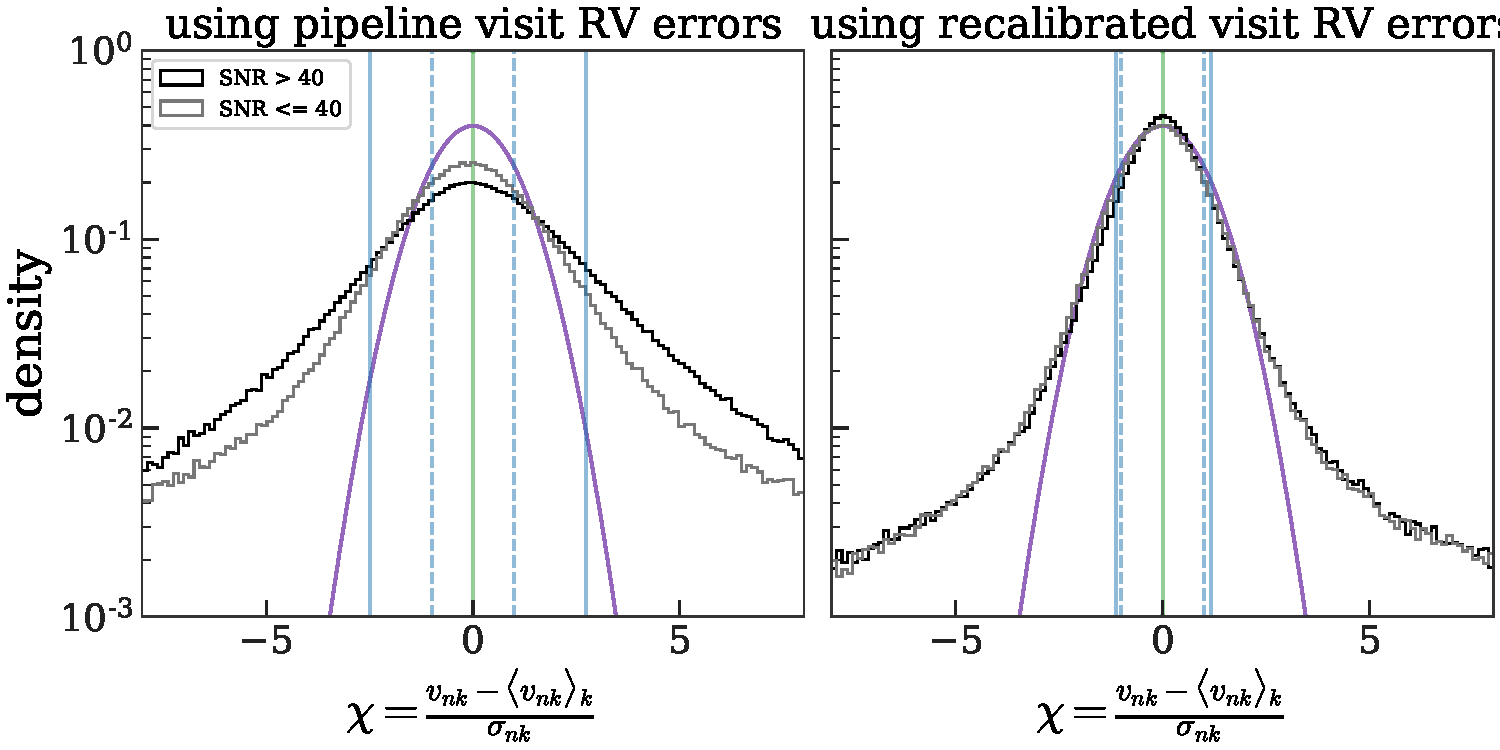
\includegraphics[width=\textwidth]{chi-distr.pdf}
\end{center}
\caption{%
TODO
\label{fig:chiplots}
}
\end{figure}


% Visit-error-calibrate.ipynb
\begin{figure}[!t]
\begin{center}
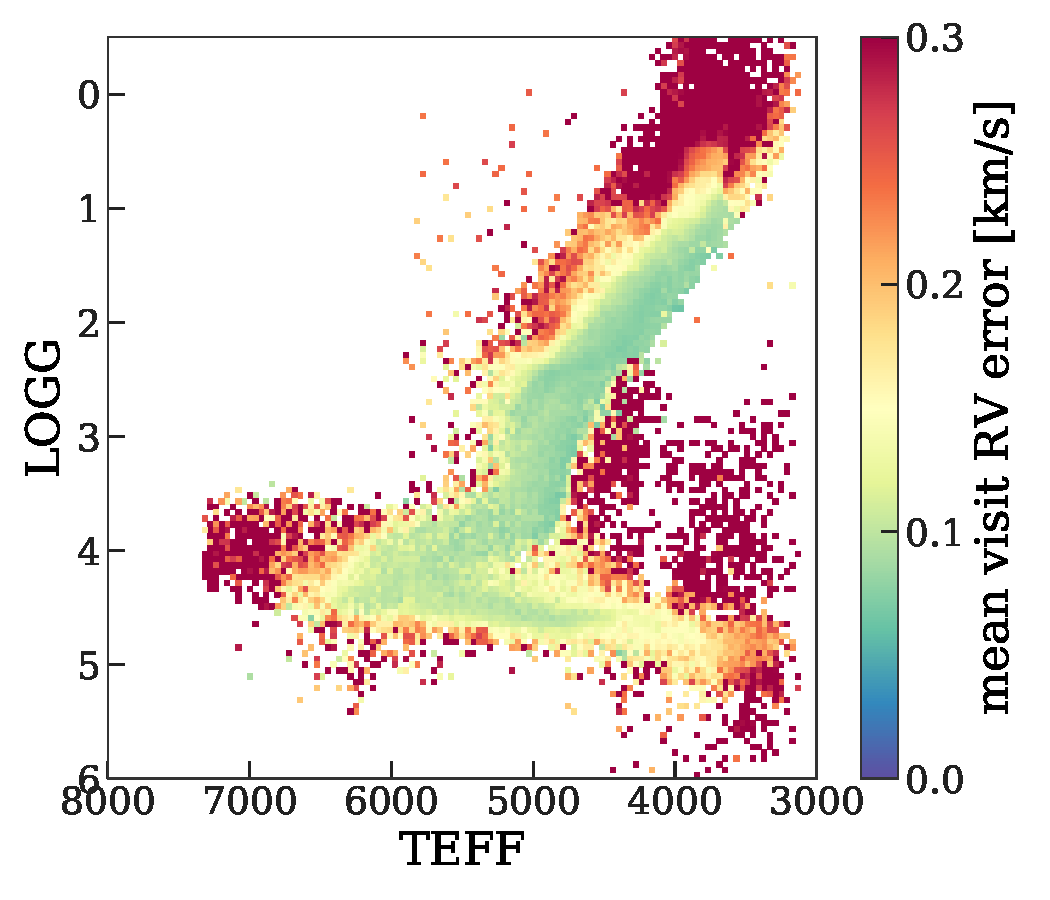
\includegraphics[width=0.7\textwidth]{mean-visit-rv-err.pdf}
\end{center}
\caption{%
TODO
\label{fig:mean-rv-err}
}
\end{figure}



\acknowledgements

It is a pleasure to thank

% APW acknowledgements support and space from the Max-Planck-Institut f\"ur
% Astronomie during initial work on this project.
% We thank the anonymous referee for constructive comments that improved this
% manuscript.

Funding for the Sloan Digital Sky Survey IV has been provided by the Alfred P.
Sloan Foundation, the U.S. Department of Energy Office of Science, and the
Participating Institutions. SDSS-IV acknowledges support and resources from the
Center for High-Performance Computing at the University of Utah. The SDSS web
site is www.sdss.org.

SDSS-IV is managed by the Astrophysical Research Consortium for the
Participating Institutions of the SDSS Collaboration including the Brazilian
Participation Group, the Carnegie Institution for Science, Carnegie Mellon
University, the Chilean Participation Group, the French Participation Group,
Harvard-Smithsonian Center for Astrophysics, Instituto de Astrof\'isica de
Canarias, The Johns Hopkins University, Kavli Institute for the Physics and
Mathematics of the Universe (IPMU) / University of Tokyo, Lawrence Berkeley
National Laboratory, Leibniz Institut f\"ur Astrophysik Potsdam (AIP),
Max-Planck-Institut f\"ur Astronomie (MPIA Heidelberg), Max-Planck-Institut
f\"ur Astrophysik (MPA Garching), Max-Planck-Institut f\"ur Extraterrestrische
Physik (MPE), National Astronomical Observatories of China, New Mexico State
University, New York University, University of Notre Dame, Observat\'ario
Nacional / MCTI, The Ohio State University, Pennsylvania State University,
Shanghai Astronomical Observatory, United Kingdom Participation Group,
Universidad Nacional Aut\'onoma de M\'exico, University of Arizona, University
of Colorado Boulder, University of Oxford, University of Portsmouth, University
of Utah, University of Virginia, University of Washington, University of
Wisconsin, Vanderbilt University, and Yale University.

This work has made use of data from the European Space Agency (ESA) mission
{\it Gaia} (\url{https://www.cosmos.esa.int/gaia}), processed by the {\it Gaia}
Data Processing and Analysis Consortium (DPAC,
\url{https://www.cosmos.esa.int/web/gaia/dpac/consortium}). Funding for the DPAC
has been provided by national institutions, in particular the institutions
participating in the {\it Gaia} Multilateral Agreement.

\software{
    Astropy \citep{astropy, astropy:2018},
    apred \citep{Nidever:2015},
    ASPCAP \citep{ASPCAP},
    exoplanet \citep{exoplanet:exoplanet},
    gala \citep{gala},
    IPython \citep{ipython},
    numpy \citep{numpy},
    pymc3 \citep{Salvatier2016},
    schwimmbad \citep{schwimmbad:2017},
    scipy \citep{scipy},
    theano \citep{theano},
    thejoker \citep{thejoker, Price-Whelan:2019a}
}


\appendix

% \section{Data tables}
% \label{sec:datatables}

% The primary data product released with this \documentname\ are the posterior
% samplings generated for each of \nsources\ sources in \apogee\ \dr{16};
% \changes{These samplings will be released in the upcoming intermediate SDSS data
% release ``DR16+'' (expected in mid-2020).}
% However, we also compute summary information and statistics aboutf these
% samplings and provide these data in \tablename~\ref{tbl:metadata}.
% We also define a \goldsample\ of high-quality, uniquely solved binary-star
% systems (see \sectionname~\ref{sec:gold-sample}) and release summary information
% along with cross-matched data from \gaia\ \dr{2} and the \acronym{STARHORSE}
% catalog of stellar parameters in \tablename~\ref{tbl:goldsample}.

% \input{tables/metadata-schema.tex}

% \input{tables/goldsample-schema.tex}

\bibliographystyle{aasjournal}
\bibliography{dr17binaries}

\end{document}
